\documentclass{article}
%\usepackage[a4paper, total={6in, 8in}]{geometry}
\usepackage{graphics}
\usepackage{geometry}
 \geometry{
 a4paper,
 total={210mm,297mm},
 left=20mm,
 right=20mm,
 top=-2mm,
 bottom=2mm,
 }
%\usepackage[margin=0.5in]{geometry}

\usepackage{amsmath,amssymb}
\usepackage{ifpdf}
%\usepackage{cite}
\usepackage{algorithmic}
\usepackage{array}
\usepackage{mdwmath}
\usepackage{pdfpages}
\usepackage{mdwtab}
\usepackage{eqparbox}
%\onecolumn
%\input{psfig}
\usepackage{color}
\usepackage{graphicx}
\setlength{\textheight}{23.5cm} \setlength{\topmargin}{-1.05cm}
\setlength{\textwidth}{6.5in} \setlength{\oddsidemargin}{-0.5cm}
\renewcommand{\baselinestretch}{1}
\pagenumbering{arabic}
\usepackage{listings}
\usepackage{xcolor}
 
\definecolor{codegreen}{rgb}{0,0.6,0}
\definecolor{codegray}{rgb}{0.5,0.5,0.5}
\definecolor{codepurple}{rgb}{0.58,0,0.82}
\definecolor{backcolour}{rgb}{0.95,0.95,0.92}
 
\lstdefinestyle{mystyle}{
    backgroundcolor=\color{backcolour},   
    commentstyle=\color{codegreen},
    keywordstyle=\color{magenta},
    numberstyle=\tiny\color{codegray},
    stringstyle=\color{codepurple},
    basicstyle=\ttfamily\footnotesize,
    breakatwhitespace=false,         
    breaklines=true,                 
    captionpos=b,                    
    keepspaces=true,                 
    numbers=left,                    
    numbersep=5pt,                  
    showspaces=false,                
    showstringspaces=false,
    showtabs=false,                  
    tabsize=2
}
\lstset{style=mystyle}
 
\begin{document}

\textbf{
\begin{center}
{
\large{School of Engineering and Applied Science (SEAS) \\ Ahmedabad University}\vspace{5mm}
}
\end{center}
%
\begin{center}
\large{BTech(ICT) Semester VI:Digital Signal Processing\\ \vspace{4mm}
Laboratory Assignment-8\\\vspace{2mm}
Enrollment No:AU1841131 \hspace{6cm} Name:Mansi Dobariya  }
\end{center}}
\vspace{2mm}

\textbf{AIM ::} LAB8  helps to understand the concept of  butterworth filter  Using \textbf{freq and butter,lp2bp} functions. In addition to this, I can use function for finding n,cutoffFreq,numerator and denominator coefficients and after that use of freqz function for plot magnitude and phase . 


\begin{enumerate}
%Q1
\item \large  \\
\textbf{Solution Problem-1 By hand written calculation}
\begin{enumerate}

	\item Matlab Script: 
	\begin{lstlisting}[language=Matlab]
clc ;
close all ;
clear ;
%impz(b,a,n) with no output arguments plots the impulse response of the digital filter with numerator coefficients b and denominator coefficients a.
%b :: coefficients of numerator part as [...b4(Z^4) b3(Z^3) b1(Z^2) b1(Z^1) b0(Z^0) b(-1)(Z^-1) b(-2)(Z^-2) b(-3)(Z^-3) ..]
%a :: coefficients of denominator part as [...b4(Z^4) b3(Z^3) b1(Z^2) b1(Z^1) b0(Z^0) b(-1)(Z^-1) b(-2)(Z^-2) b(-3)(Z^-3) ..]
b=[0.1067 -0.4267 0.64 -0.4266 0.1067];
a=[1 -0.1467 0.4931 -0.03112 0.018184];

%freqz function : freqz(b,a,n,fs) without output argument,Display the magnitude and phase responses of the filter.
%b :: numerator coefficients
%a :: denominator coefficients
%(optional)n :: Number of evaluation points, specified as a positive integer scalar no less than 2. When n is absent, it defaults to 512. For best results, set n to a value greater than the filter order.
%fs :: sampling freq
fs=1000;
figure(1)
freqz(b,a,fs);
title('By hand Written')

\end{lstlisting}
\\	
    \item Approach:\\
    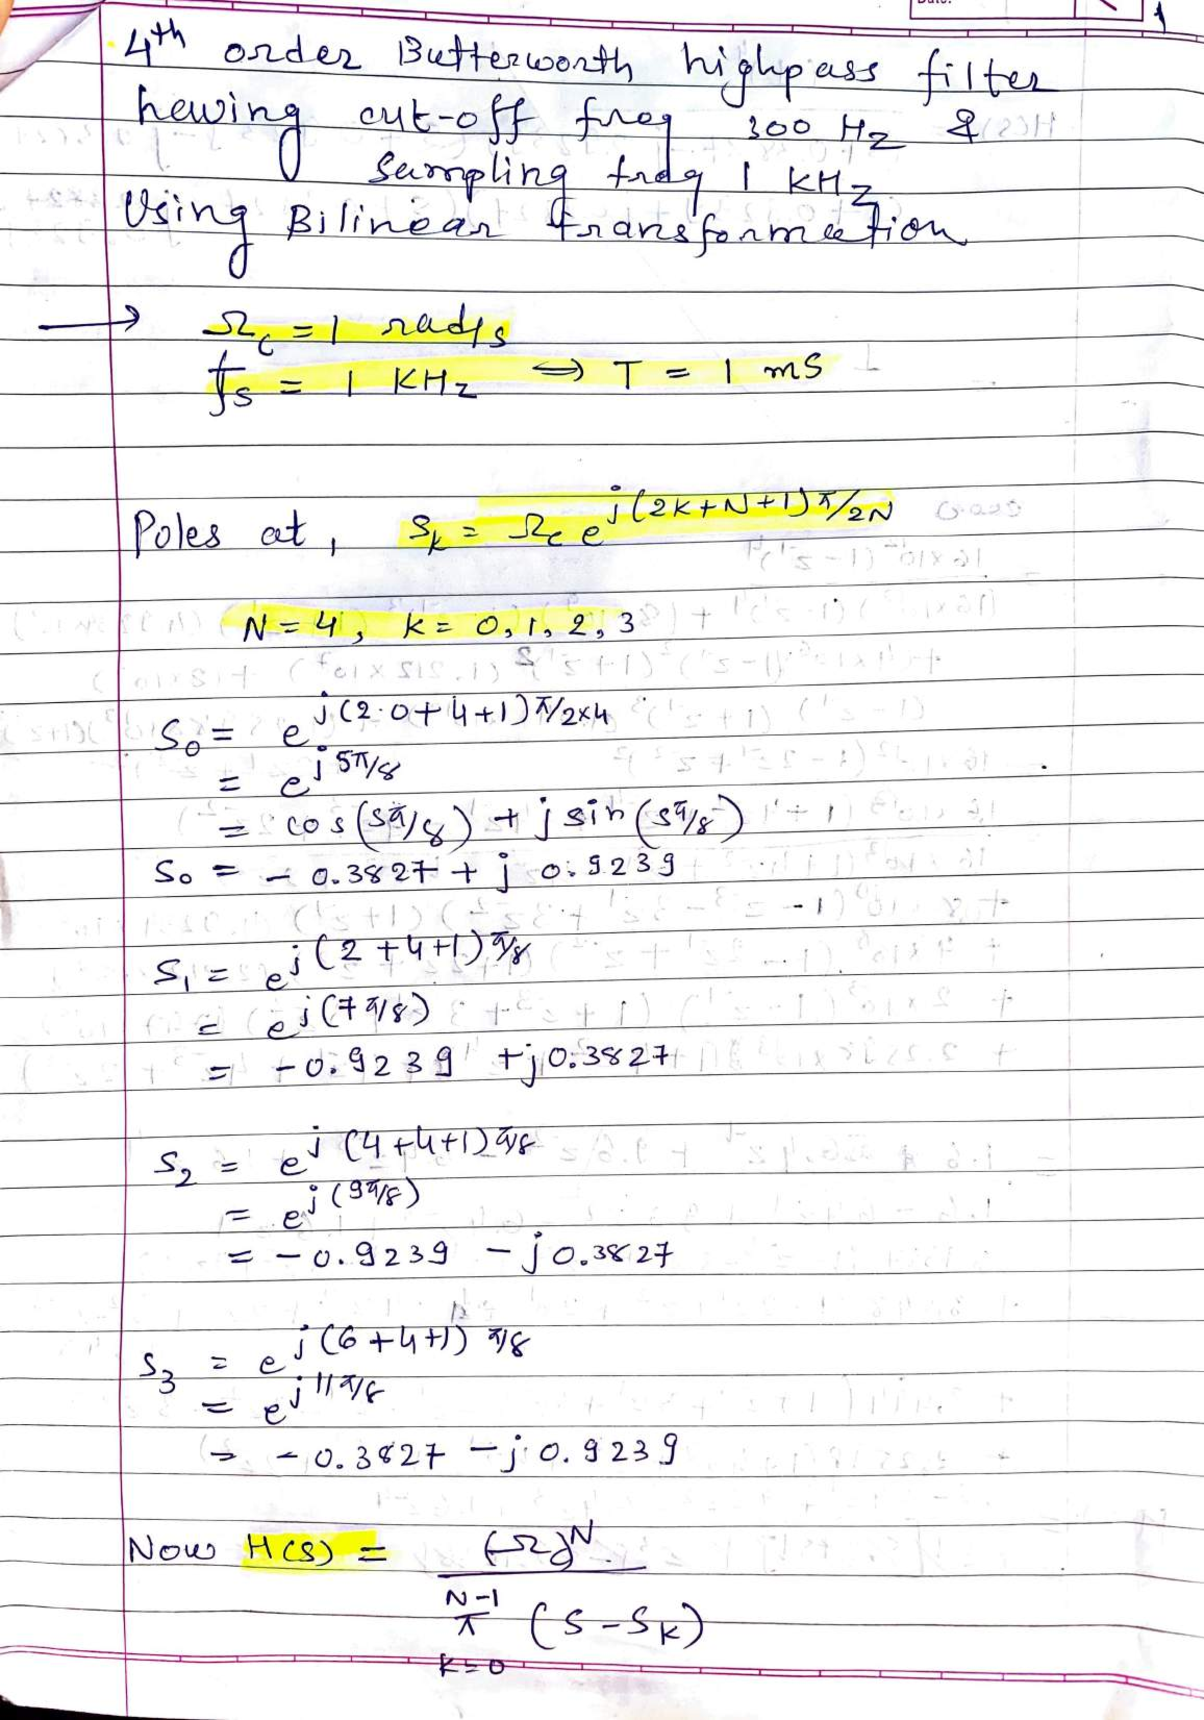
\includepdf[pages=-]{dsp_last-compressed.pdf}
   \\

	\begin{center}
    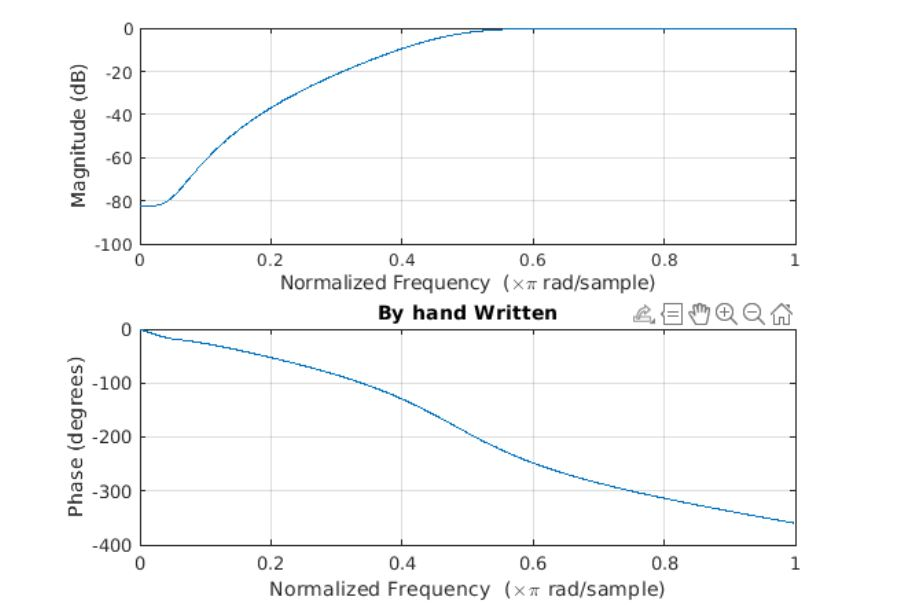
\includegraphics[width=0.9\textwidth]{A9_1_1.JPG}
    \end{center}
\end{enumerate}	
\\
%\end{enumerate}

\item \large  \\
\textbf{Solution Problem-1 using butter and lp2hp function}
\begin{enumerate}

	\item Matlab Script: 
	\begin{lstlisting}[language=Matlab]
clc ;
close all ;
clear ;
% Bilinear transformation using fucntions============================================
%high cutoff frequency fc = 300Hz so wc =2*pi*fc => 600*pi and sampling f=1000
N=4;% order N = 4
fc=300;
wc=2*pi*fc;
[b,a] = butter (N, 1,"low", 's');
% converting from LP filter to HP filter
% We get high pass analog filter transfer function coefficients bt and at
[bt, at] = lp2hp (b, a, wc);
fs=10^3;
[bz, az] = bilinear (bt, at, fs) ;
%b :: coefficients of numerator part as [...b4(Z^4) b3(Z^3) b1(Z^2) b1(Z^1) b0(Z^0) b(-1)(Z^-1) b(-2)(Z^-2) b(-3)(Z^-3) ..]
%a :: coefficients of denominator part as [...b4(Z^4) b3(Z^3) b1(Z^2) b1(Z^1) b0(Z^0) b(-1)(Z^-1) b(-2)(Z^-2) b(-3)(Z^-3) ..]
% Plot the zeros and poles
figure(1)
freqz(bz,az)
figure(2)
zplane (bz,az);
\end{lstlisting}
\\	
    \item Approach:\\
  With order 4 ,sampling time =0.001,High pass cutoof frq 300Hz. Using this as arguments in butter fucntion to find transfer function coeeficents to lowpass in S domain.Passing this coefficietns to lp2bp to get high pass filter's coeficients function ,Passing output of this in bilinear transformation function bilinear to get Z-domain's coefficients.At the end plotted into freqz and zero and poles.
   \\

	\begin{center}
    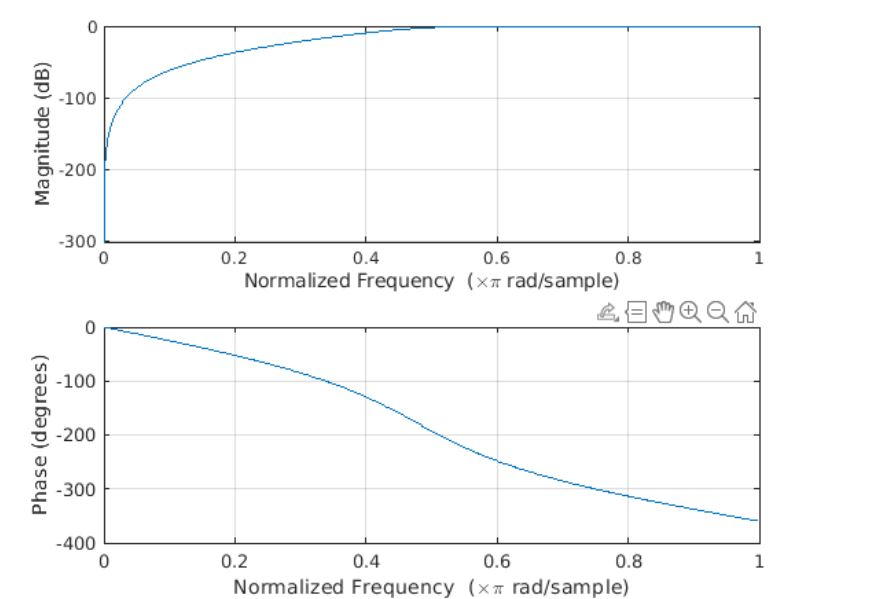
\includegraphics[width=0.9\textwidth]{A9_1_3.JPG}
    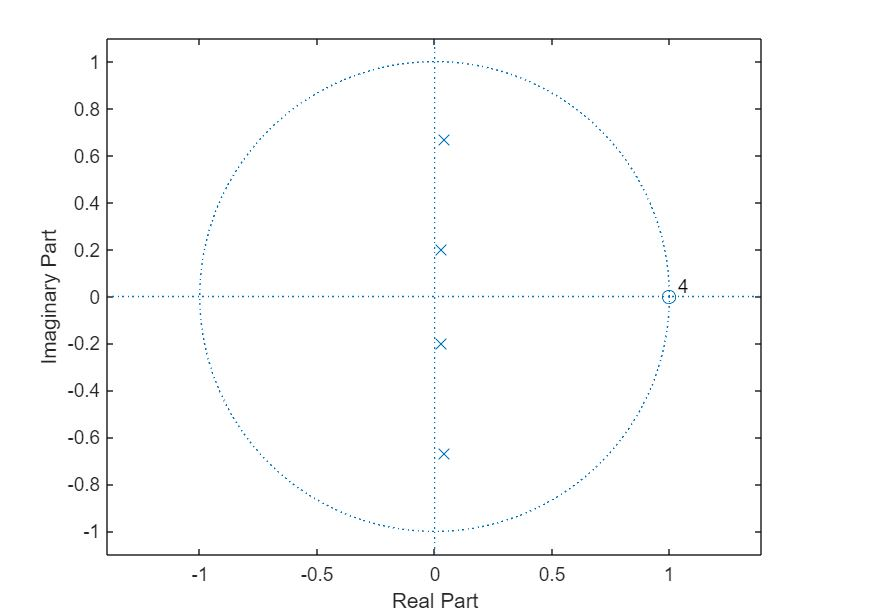
\includegraphics[width=0.9\textwidth]{A9_1_2.JPG}
    \end{center}
\end{enumerate}	
\\
%\end{enumerate}

\end{enumerate}

\end{document} 